\documentclass[13pt,oneside]{book}
\usepackage[utf8]{inputenc}
\usepackage{url}
\usepackage{graphicx}

\usepackage{geometry}
\geometry{a4paper, left=20mm, right=20mm, top=20mm, bottom=20mm}
\usepackage[margin=1.2in]{geometry}
\usepackage[toc,page]{appendix}
\usepackage{graphicx}
\usepackage{natbib}
\usepackage{lipsum}
\usepackage{caption}

\begin{document}

\captionsetup[figure]{margin=1.5cm,font=small,labelfont={bf},name={Figure},labelsep=colon,textfont={it}}
\captionsetup[table]{margin=1.5cm,font=small,labelfont={bf},name={Table},labelsep=colon,textfont={it}}
\setlipsumdefault{1}

\begin{titlepage}
\begin{center}
{\LARGE College Of Engineering Trivandrum}\\[3cm]
\linespread{1.2}\huge {\bfseries Application Software Development Lab}\\[3cm]
\linespread{1}

\includegraphics[width=5cm]{img/emblem.jpeg}\\[3cm]
{\Large GOKUL K\\ S5  CSE \\ Roll No:21\\ TVE18CS021 }\\[1cm]


\textit{ }\\[2cm]
Department of Computer Science\\[0.2cm]
\today
\end{center}

\end{titlepage}

\newpage

\begin{frame}{}
    \centering
    \hspace*{-0.5cm}
    $\vcenter{\hbox{
\includegraphics[width=1.5cm]{img/emblem.jpeg}}}$
    $\vcenter{\resizebox{0.95\textwidth}{!}{
        \begin{tabular}{c}
             CS333 - Application Software Development Lab $\cdot$ 2020 $\cdot$   \\
             \hline 
        \end{tabular}
    }}$
\end{frame}
\section*{Cycle 1}
\section*{Expt 2}
\begin{center}
    \Large{Basic SQL Queries - I}
\end{center}

\section*{Aim}
\large{To study the basic queries such as
	\begin{enumerate}
		\item SELECT
		\item INSERT
		\item UPDATE
		\item DELETE
	\end{enumerate}
}

\section*{Experiment}
	\begin{enumerate}
		\item 
			Insert records into the employee table (Fields : EmpId, Ename,
Designation, Salary, Dept.id) created.
            
             Synatx:
			\begin{verbatim}
CREATE TABLE Employee(
	Emp_no INT(6) PRIMARY KEY,
	Ename VARCHAR(10),
	Designation VARCHAR(10),
	Salary INT(6),
	Dept_id INT(4)
);

INSERT INTO Employee
VALUES
	(66928, "BLAZE", "MANAGER", 55000, 3001),
	(67832, "CLARE", "MANAGER", 51000, 1001),
	(65646, "JONAS", "MANAGER", 59140, 2001),
	(67858, "SCARLET", "ANALYST", 62000, 2001),
	(69062, "FRANK", "ANALYST", 62000, 2001),
	(63679, "SANDRINE", "CLERK", 18000, 3001),
	(64989, "ADELYN", "SALESMAN", 34000, 3001),
	(65271, "WADE", "SALESMAN", 27000, 3001),
	(66564, "MADDEN", "SALESMAN", 27000, 3001),
	(68454, "TUCKER", "SALESMAN", 32000, 3001),
	(68736, "ANDRES", "CLERK", 24000, 2001),
	(69000, "JULIUS", "CLERK", 21000, 3001),
	(69324, "MARKER", "CLERK", 28000, 1001);
			\end{verbatim}
			\includegraphics{1.jpg}
		
			\item 
			Display the details of all the employees.
			
			Syntax:
			\begin{verbatim}
SELECT * FROM Employee;
			\end{verbatim}
			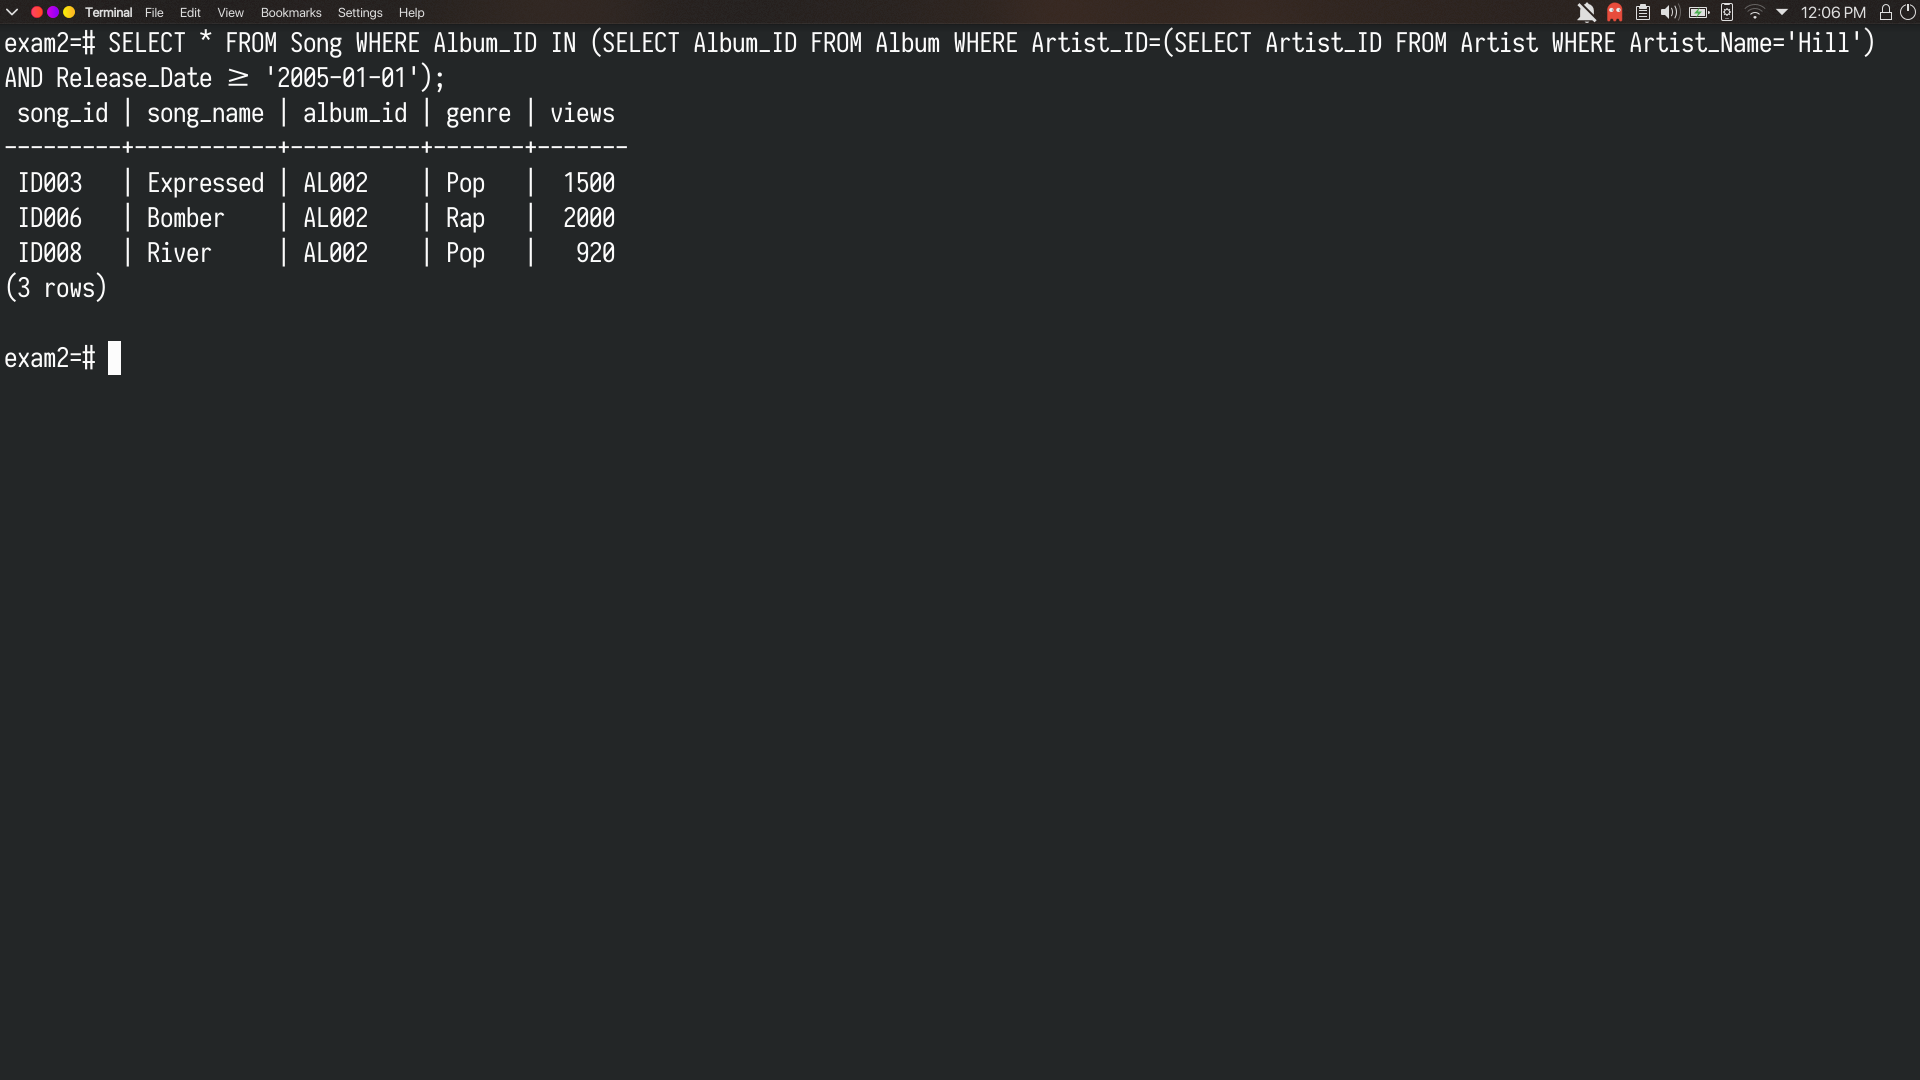
\includegraphics{2.JPG}
		
		\item 
		Display the employee numbers, names and designation of all employees.
		
		Syntax:
		\begin{verbatim}
SELECT Emp_no, Ename, Designation
FROM Employee;
		\end{verbatim}
		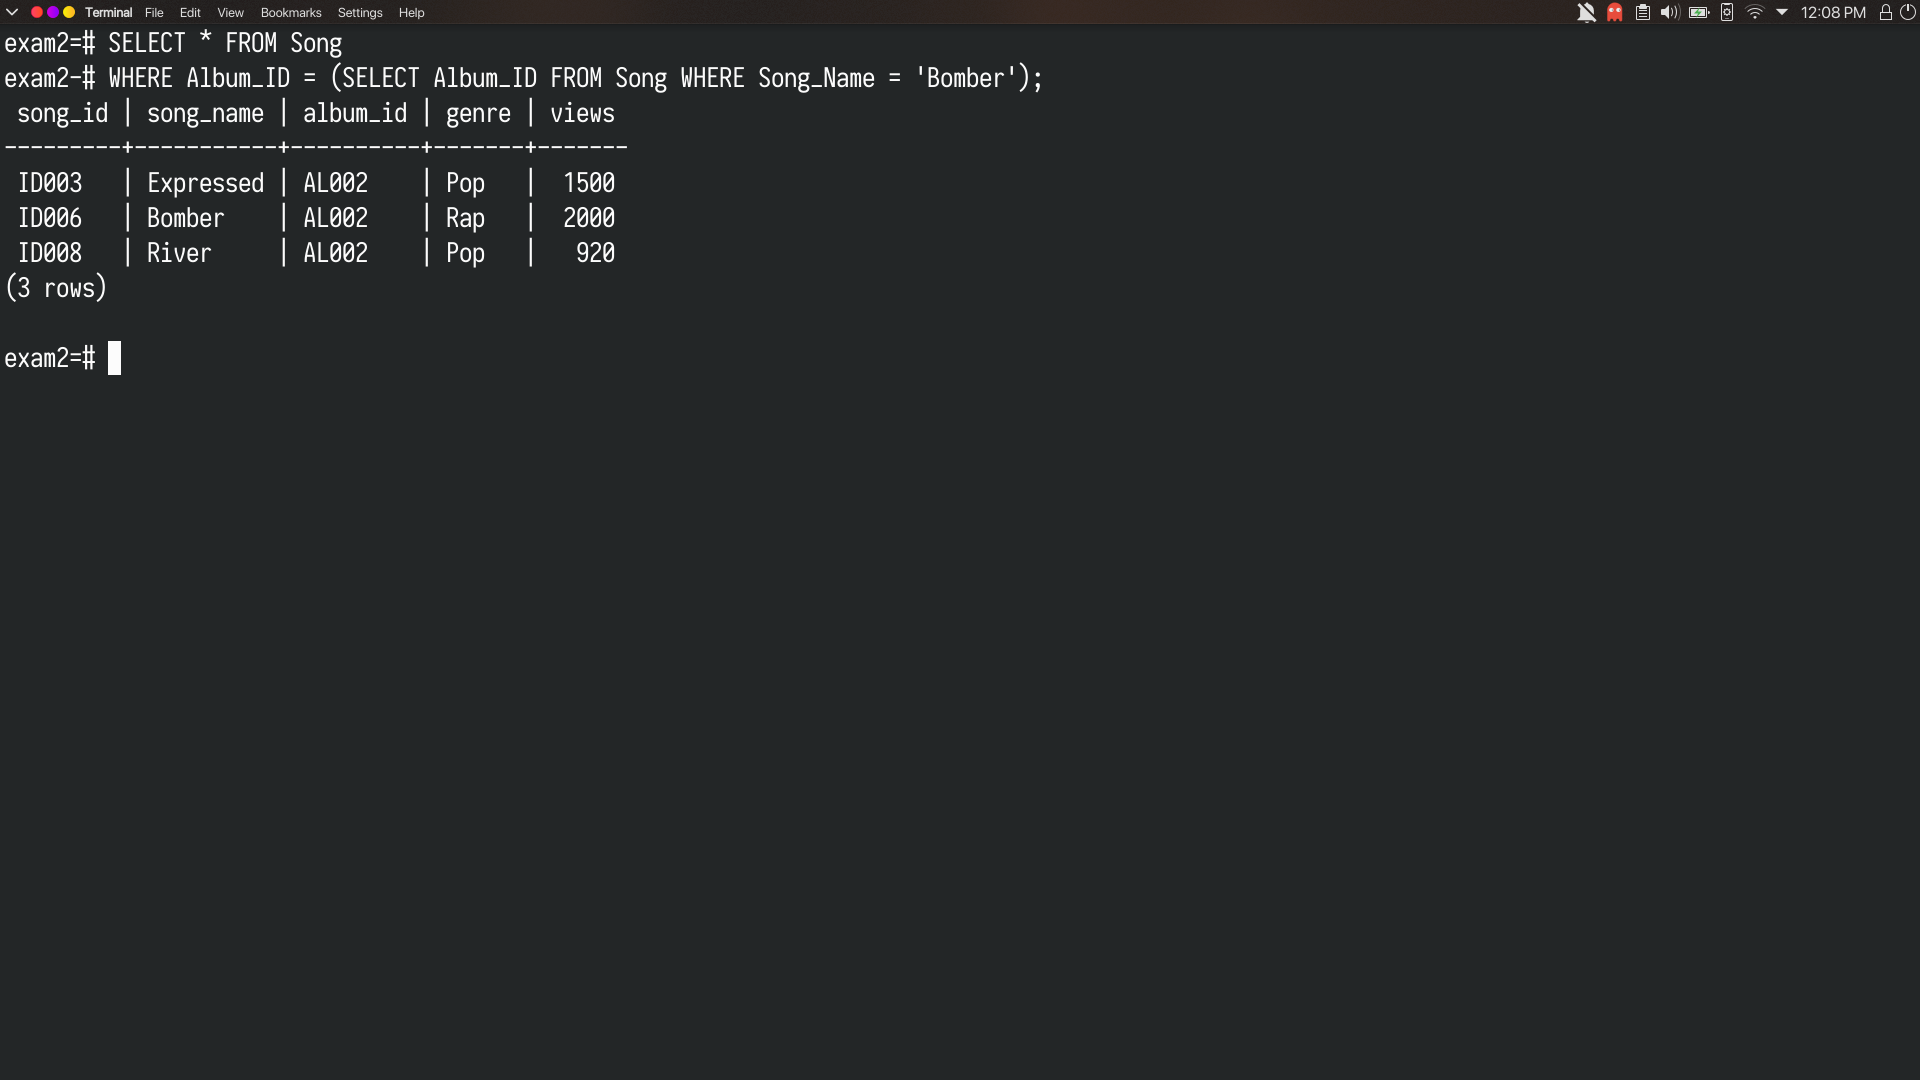
\includegraphics{3.jpg}

		\item
		Suppose the emp\_no 68454 has left the company. Delete the employee
from the database.
		Syntax: 
		\begin{verbatim}
DELETE FROM Employee
WHERE Emp_no=68454;
		\end{verbatim}
	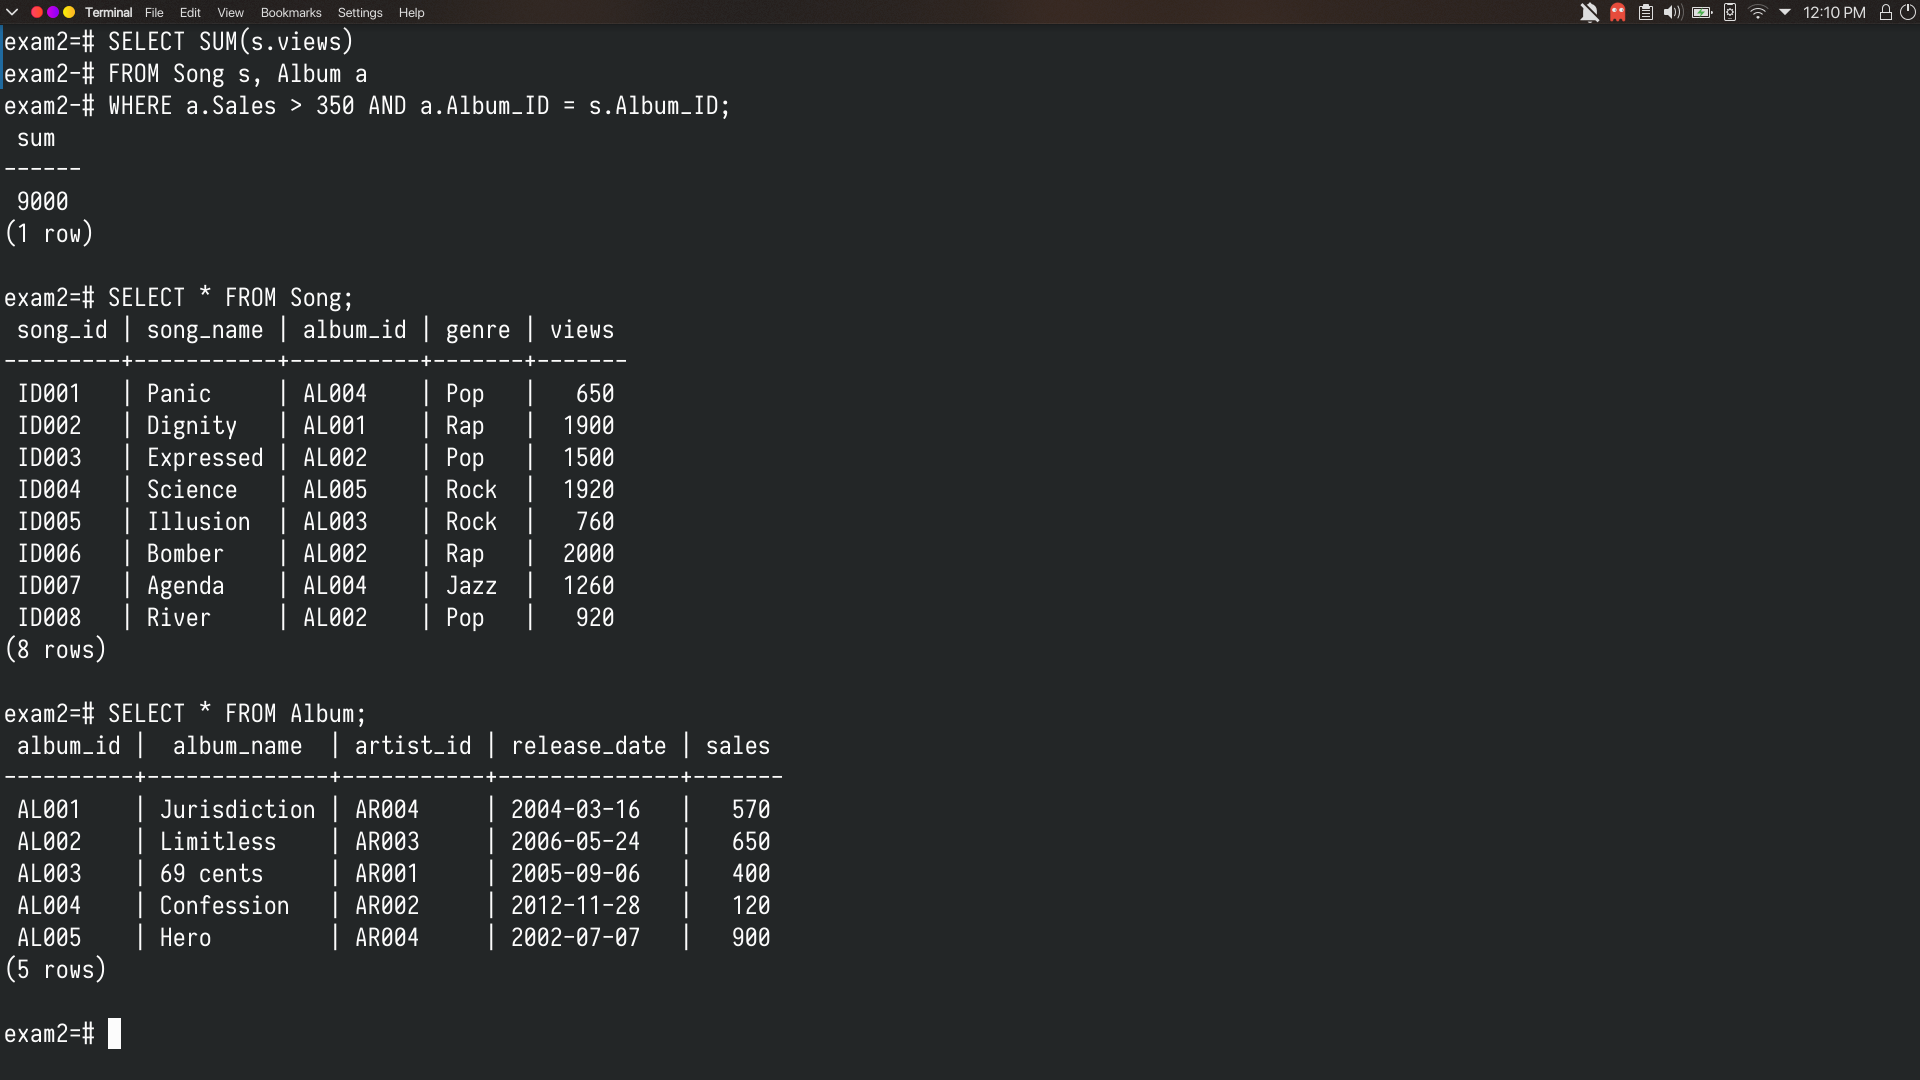
\includegraphics{4.jpg}
    
    \item
    Suppose a new employee joins the company under department 2001 as
an analyst. The salary of the employee is not yet fixed. Add his record to
the database.

    Syntax:
    \begin{verbatim}
INSERT INTO Employee
(Emp_no, Ename, Designation, Dept_id) VALUES
	(69876, "Rahul", "ANALYST", 2001);
    \end{verbatim}
    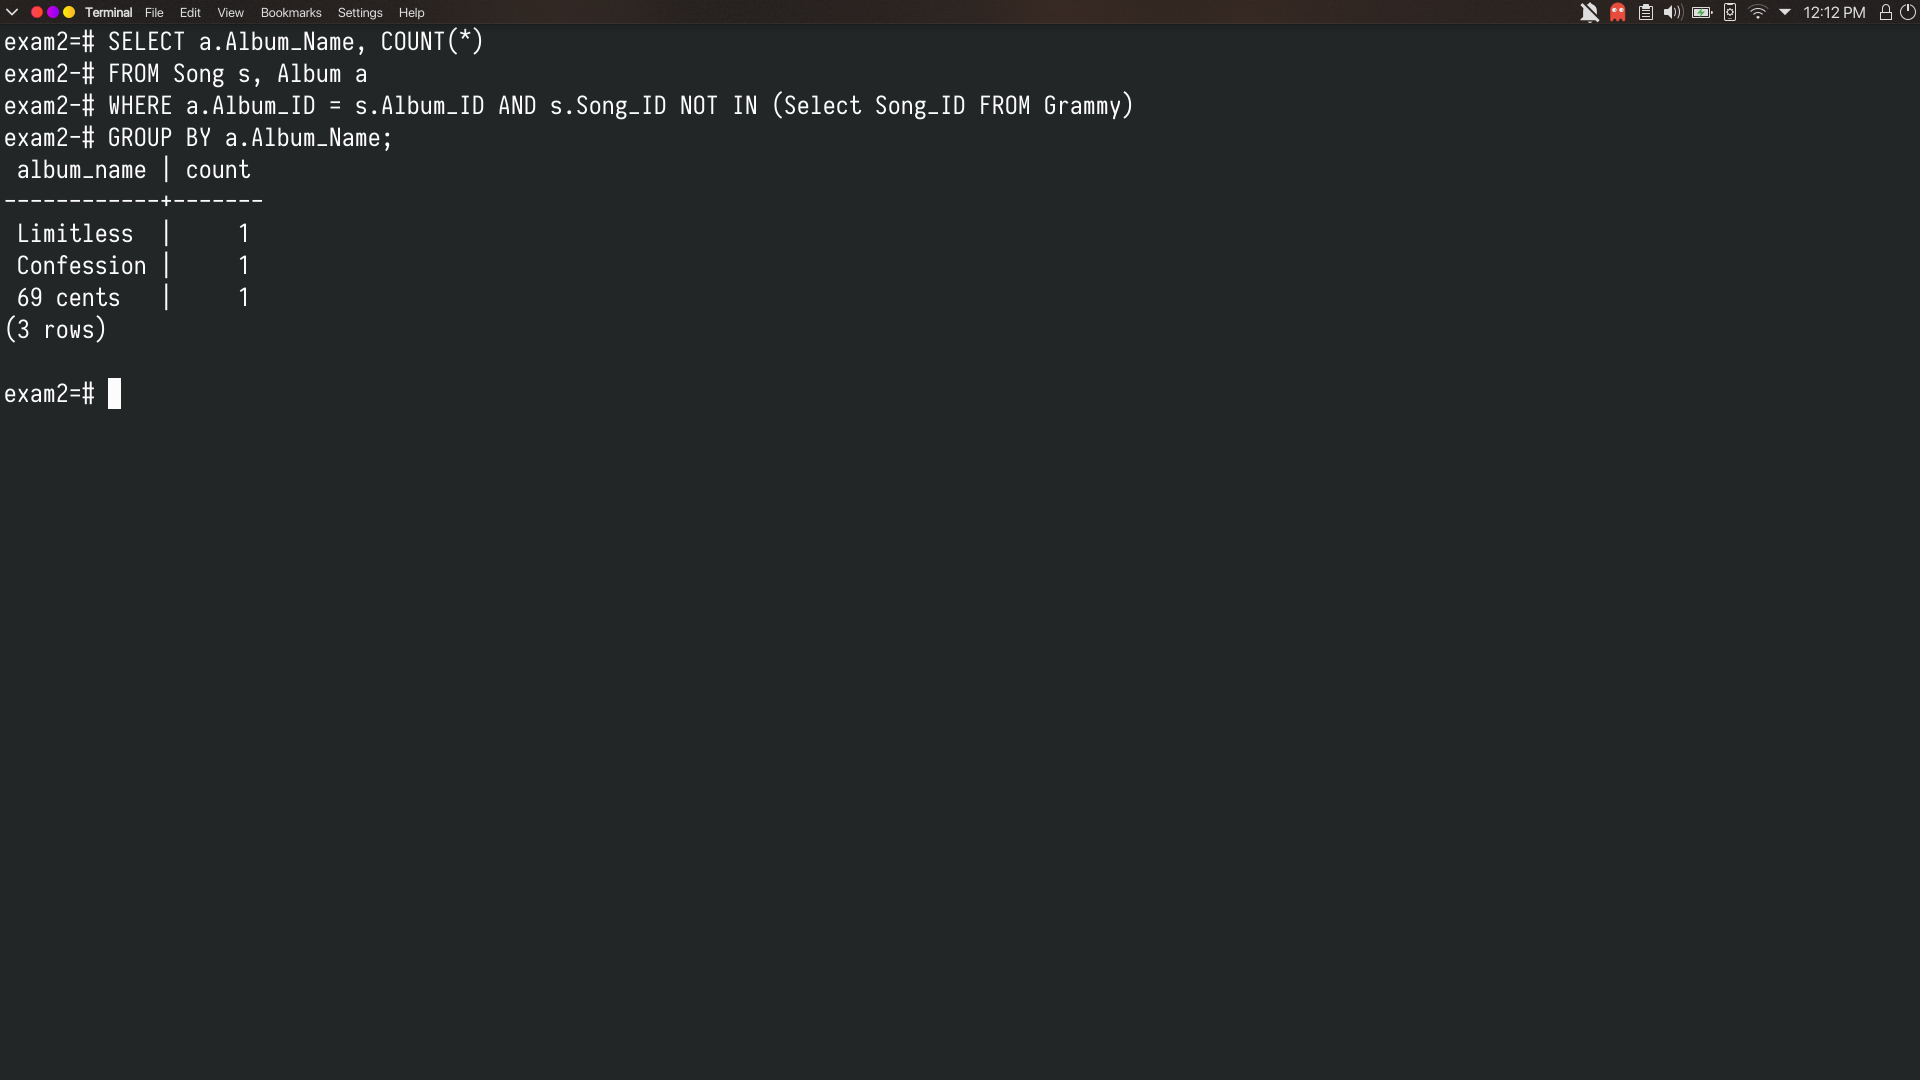
\includegraphics[]{5.jpg}

\item
Find the details of employees with salary > 25000 working in department
with id 2001.

Syntax:
\begin{verbatim}
SELECT * FROM Employee
WHERE Salary>25000 AND Dept_id=2001;
\end{verbatim}
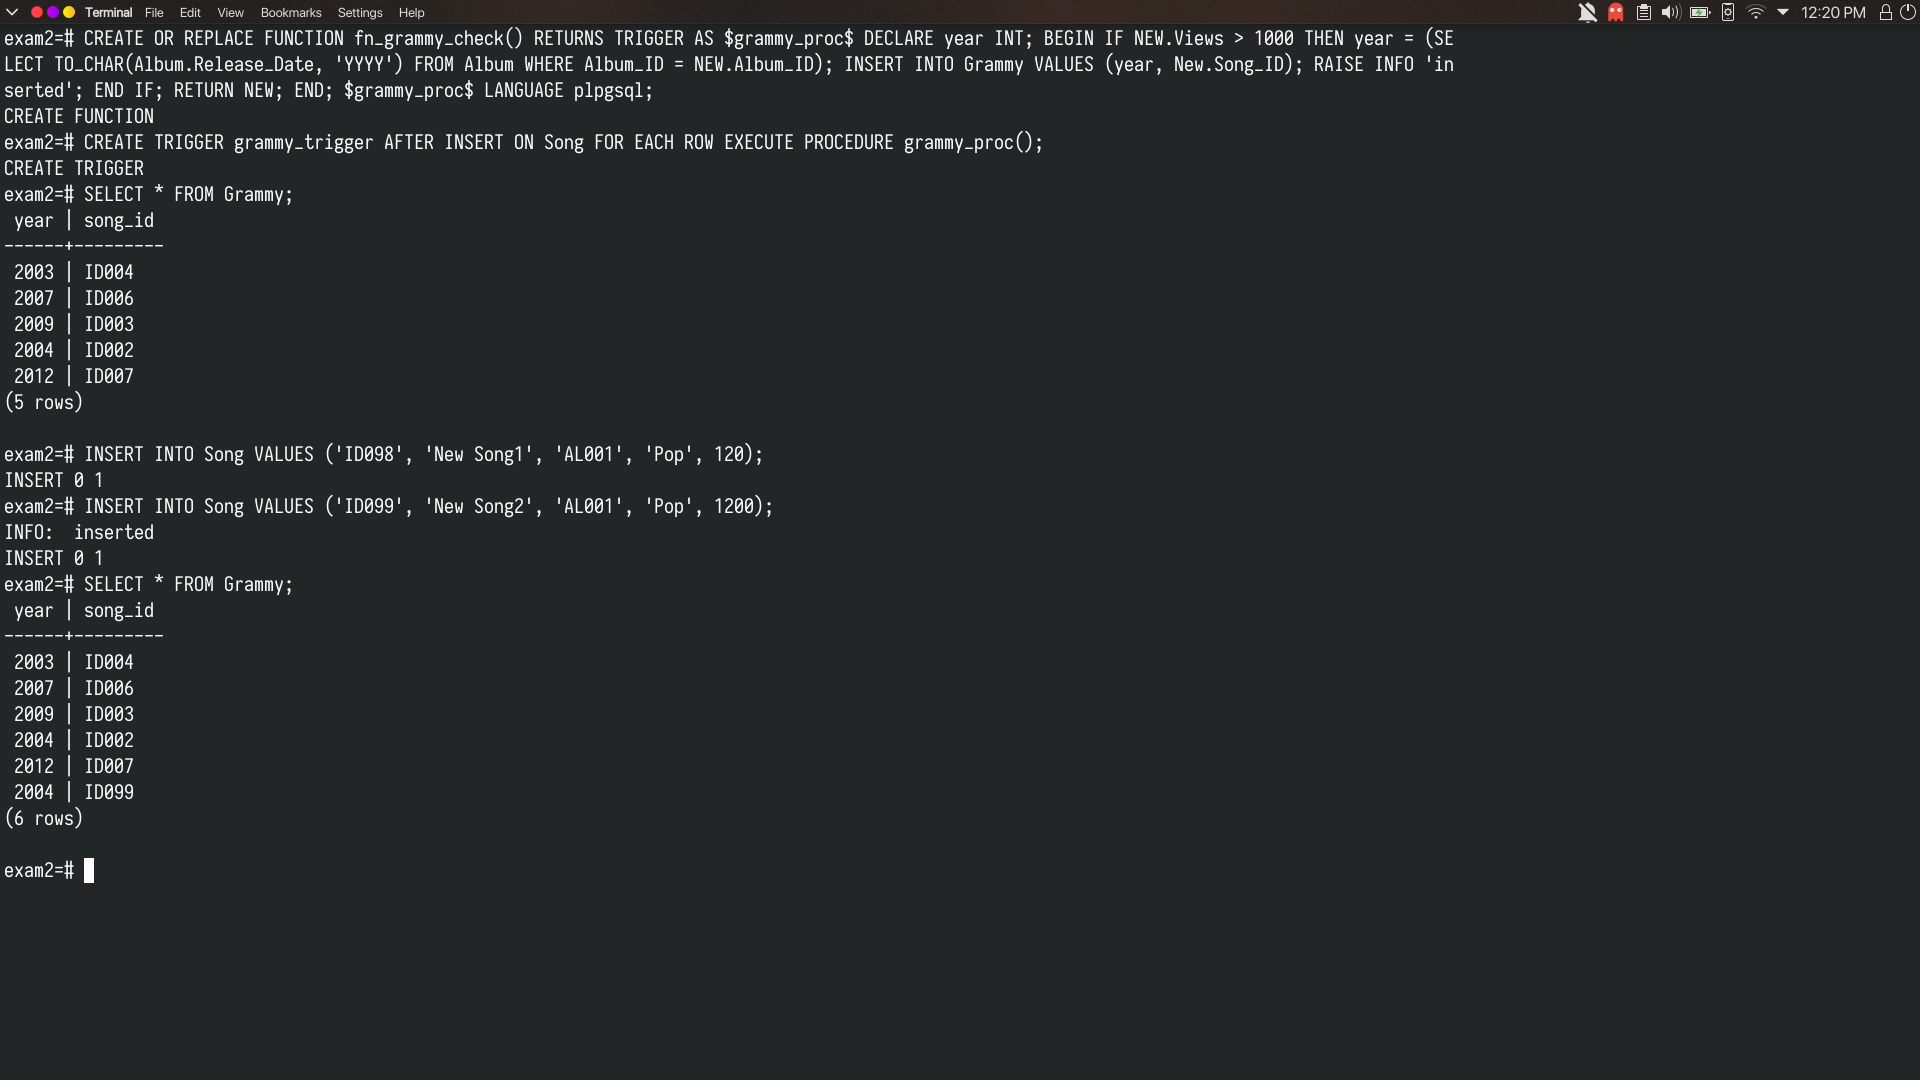
\includegraphics[]{6.jpg}

\item
		Suppose the newly added employee's salary is now fixed. Add his salary
details.
		Syntax: 
		\begin{verbatim}
UPDATE Employee
SET Salary=40000
WHERE Emp_no=69876;
		\end{verbatim}
		\includegraphics{img/p2/ssg}
		
	\item
	Suppose the employee ADELYN is now promoted as Analyst. Update his
designation and salary.
Syntax:
    \begin{verbatim}
UPDATE Employee
SET Designation="ANALYST", Salary=40000
WHERE Ename="ADELYN";
    \end{verbatim}
	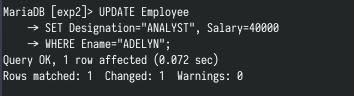
\includegraphics[]{img/p2/ss8.png}
	
	\item
	Display the names of all managers and analysts.
Syntax:
    \begin{verbatim}
SELECT * FROM Employee
WHERE Designation="MANAGER" OR Designation="ANALYST";
    \end{verbatim}
	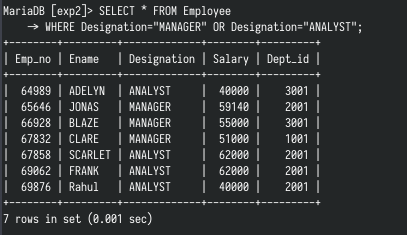
\includegraphics[]{img/p2/ss9.png}
	
		\item
Retrieve the names of all employees whose salary is between 30000
and 60000.
    \begin{verbatim}
SELECT * FROM Employee
WHERE Salary>30000 AND Salary<60000;
    \end{verbatim}
	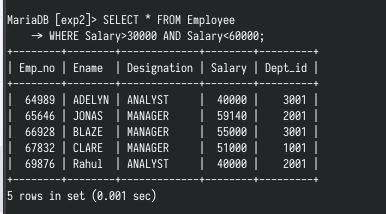
\includegraphics[]{img/p2/ss10.png}
	
		\item
A salary hike is now announced by dept. 2001. Update the salary of all
their employees by 5\%.

    \begin{verbatim}
UPDATE Employee
SET Salary = Salary + Salary*(0.05)
WHERE Dept_id=2001;
    \end{verbatim}
	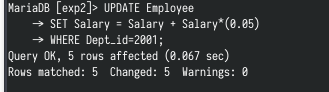
\includegraphics[]{img/p2/ss11.png}
	
			\item
List all employees whose salary is less than 30000 or working for dept.
1001.

    \begin{verbatim}
SELECT * FROM Employee
WHERE Salary<30000 OR Dept_id=1001;

    \end{verbatim}
	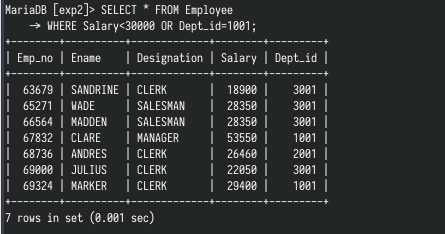
\includegraphics[]{img/p2/ss12.png}
	
	\end{enumerate}
	\section*{Result}
	The basic SQL for creating and modifying a table is executed and their output
	is verified in a MySQL environment.
\end{document}